% Slides: mbirtorch features added since release v0.0.2, and the high-value
% features of LEAP and TIGRE that mbirtorch still lacks.
% Same look and feel as the pcdrecon decks (research_notes/decks/ in that
% repository).  Build: latexmk mbirtorch_update_deck.tex (see latexmkrc).
% Figures: make_figures.py writes the charts into images/ and copies the
% images it can reach; README.md names the source of every image.
%
% Every feature slide has three parts: the problem, what changed, how to use
% it.  Every gap slide has four: the gap for a user, what LEAP and TIGRE have,
% what mbirtorch has today, what is needed.  Text sits on the left and the
% figure on the right.
\documentclass[aspectratio=169,10pt]{beamer}
\usepackage[T1]{fontenc}
\usepackage[utf8]{inputenc}
\usetheme[progressbar=frametitle,numbering=fraction]{metropolis}
\usepackage[sfdefault,lining]{FiraSans}
\usepackage{FiraMono}
\usepackage{graphicx}
\usepackage{array}
\usepackage{colortbl}
\usepackage{calc}
\usepackage{tikz}
\usetikzlibrary{positioning,arrows.meta,calc}
\graphicspath{{images/}}

% One accent for the deck itself; the chips get their own colors.
\definecolor{planAccent}{HTML}{3D6B99}   % stats, note bars, mbirtorch
\definecolor{safeGreen}{HTML}{2E7D32}    % released
\definecolor{axialBrick}{HTML}{A23B3B}   % prototype, and LEAP/TIGRE bars
\definecolor{branchAmber}{HTML}{B26B1F}  % on a branch
\definecolor{leapPurple}{HTML}{6B4C9A}   % LEAP chips
\definecolor{tigreTeal}{HTML}{1F7A8C}    % TIGRE chips
\definecolor{inkGray}{HTML}{5A5A5A}
\definecolor{barGray}{HTML}{262626}

\setbeamercolor{frametitle}{bg=barGray, fg=white}

% Chips in the frame title bar.
\newcommand{\tagchip}[2]{{\setlength{\fboxsep}{2.5pt}\setlength{\fboxrule}{0.6pt}%
  \fcolorbox{white}{#1}{\textcolor{white}{\footnotesize\bfseries\strut #2}}}}
\newcommand{\released}{\tagchip{safeGreen}{RELEASED}}
\newcommand{\onbranch}{\tagchip{branchAmber}{BRANCH}}
\newcommand{\prototype}{\tagchip{axialBrick}{PROTOTYPE}}
\newcommand{\leaprank}[1]{\tagchip{leapPurple}{LEAP #1}}
\newcommand{\tigrerank}[1]{\tagchip{tigreTeal}{TIGRE #1}}

\newcommand{\speclabel}[1]{\textcolor{inkGray}{\scriptsize\MakeUppercase{#1}}}

% A note with the accent bar; the bar spans the whole note.
\newsavebox{\notebox}
\newcommand{\noteline}[1]{%
  \savebox{\notebox}{\begin{minipage}[b]{0.94\linewidth}\raggedright
    {\small\textcolor{inkGray}{#1}}\end{minipage}}%
  {\color{planAccent}\rule[-\dp\notebox]{2pt}{\dimexpr\ht\notebox+\dp\notebox\relax}}%
  \hspace{6pt}\usebox{\notebox}}

% The same note bar in footnotesize, for a slide that is short of room.
\newcommand{\footnoteline}[1]{%
  \savebox{\notebox}{\begin{minipage}[b]{0.94\linewidth}\raggedright
    {\footnotesize\textcolor{inkGray}{#1}}\end{minipage}}%
  {\color{planAccent}\rule[-\dp\notebox]{2pt}{\dimexpr\ht\notebox+\dp\notebox\relax}}%
  \hspace{6pt}\usebox{\notebox}}

% A record cited at the foot of a slide.
\newcommand{\source}[1]{\par\vfill{\scriptsize\textcolor{inkGray}{Source: #1}\par}}

% A light rule between the rows of a table whose cells wrap.
\newcommand{\rowrule}{\\[3pt]\arrayrulecolor{inkGray!35}\hline\noalign{\vskip 3pt}}

% A caption under a figure.
\newcommand{\figcaption}[1]{{\scriptsize\textcolor{inkGray}{#1}\par}}

% The part headings that every feature and gap slide uses.
\newcommand{\head}[1]{\textbf{#1}}

% A feature that takes two slides: the second slide gets the accent-blue title
% bar and opens with a line that names the feature and what the slide adds.
\newenvironment{continuation}{\begingroup\setbeamercolor{frametitle}{bg=planAccent, fg=white}}{\endgroup}
\newcommand{\continued}[2]{{\small\textcolor{planAccent}{\textbf{#1, continued:} #2}}\par\vspace{5pt}}

\title{mbirtorch since v0.0.2}
\subtitle{New features, and the high-value features of LEAP and TIGRE we still lack}
\author{Greg Buzzard}
\date{September 2026}

\begin{document}

\maketitle

% ================================================================ purpose
\begin{frame}{What these slides cover}
  \medskip
  {\large Two questions: what mbirtorch gained since its last release, and
  what LEAP and TIGRE, the two most similar packages, still have that it
  lacks.}\par\vspace{6pt}
  {\small
  \textbf{Part 1, new features.}  Release v0.0.2 went to PyPI on 2026-08-21.
  One feature per slide, in three parts: the problem, what changed, and how
  to use it.  Each title carries a colored label:
  \released~means in the package on the \texttt{greg\_dev} branch, not yet on PyPI;
  \onbranch~means complete on a development branch;
  \prototype~means research code outside the package.
  A feature that needs a second slide continues under a
  \textcolor{planAccent}{\textbf{blue}} title bar and opens with a line naming
  the feature.\par\vspace{6pt}
  \textbf{Part 2, missing features.}  Two comparison documents list the LEAP
  and TIGRE features mbirtorch lacks and rank them by value to its users.  Each gap gets
  four parts: the gap for a user, what LEAP and TIGRE have, what mbirtorch
  has today, and what is needed.  Each title carries the rank each document
  gave the item, as \leaprank{1} and \tigrerank{4}.\par\vspace{6pt}
  \textbf{Every number is copied from a record} named at the foot of the slide.}
\end{frame}

% ================================================================ overview, new
\begin{frame}{New features at a glance}
  \vspace{0pt}
  {\footnotesize
  \begin{tabular}{@{}>{\raggedright\arraybackslash}p{0.24\linewidth}@{\hspace{6pt}}>{\raggedright\arraybackslash}p{0.60\linewidth}@{\hspace{6pt}}l@{}}
    \speclabel{feature} & \speclabel{what it gives a user} & \speclabel{status} \\[3pt]
    Geometry calibration & the center of rotation and the detector rotation, estimated from the sinogram & \released \\[4pt]
    Geometry viewer & a five-panel drawing of the scan, with data overlays and a comparison & \released \\[4pt]
    One geometry map & the projectors and the viewer share one voxel-to-detector map, exposed as \texttt{project\_points} & \released \\[4pt]
    Lower GPU memory & arrays in use fell from 29.0 to 24.9 GiB per GPU on a collaborators' scan & \released \\[4pt]
    Faster copy back & a reconstruction returns from the GPUs in 0.24 s instead of 5.7 s & \released \\[4pt]
    Multi-axis kernels & hand-written GPU kernels for the multi-axis model, 4.6 times faster on one GPU & \released \\[4pt]
    MACE loop and agents & a consensus loop; any image-to-image function is an agent & \onbranch \\[4pt]
    Multi-slice fusion & three network denoisers, one per slice orientation, fused with the data & \prototype \\[4pt]
    4D reconstruction & one volume per time frame from one continuous scan & \onbranch \\
  \end{tabular}}
\end{frame}

% ================================================================ overview, missing
\begin{frame}{Missing features at a glance}
  \vspace{0pt}
  {\small The two documents' rankings, merged, in the order Part 2 covers them:}\par\vspace{3pt}
  {\footnotesize
  \begin{tabular}{@{}l@{\hspace{6pt}}>{\raggedright\arraybackslash}p{0.48\linewidth}@{\hspace{6pt}}l@{\hspace{6pt}}l@{\hspace{6pt}}>{\raggedright\arraybackslash}p{0.24\linewidth}@{}}
    \speclabel{order} & \speclabel{feature} & \speclabel{leap} & \speclabel{tigre} & \speclabel{size of the work} \\[3pt]
    1 & Offset-scan and truncated-object support & 1 & 4 & two independent parts \\[3pt]
    2 & A low-memory execution mode & 2 & 5 & large; a plan exists \\[3pt]
    3 & Scatter correction & 3 & 6 & small first step \\[3pt]
    4 & Analytic phantoms and a noise simulator & 4 & 7 & small \\[3pt]
    5 & Polychromatic and dual-energy physics & 5 & -- & needs a spectrum library \\[3pt]
    6 & Per-view flexible geometry & 6 & 3 & the largest item \\[3pt]
    7 & Classical algorithms, composable priors, PICCS & 8 & 1, 2 & medium \\[3pt]
    8 & The remaining calibration utilities & 7 & -- & medium \\[3pt]
    9 & Fan beam, detector deblur, loaders, a quality hook & 9, 10 & 8, 9 & small each \\
  \end{tabular}}
  \vfill
  \noteline{The LEAP comparison ranked calibration first; it is eighth here
  because mbirtorch now has the two estimators of Part 1.  The low-memory mode
  and the physics corrections rank higher than before, on evidence from the
  ORNL scan and the ORNL collaborators' scripts.}
  \source{\texttt{plans/features/leap\_comparison/leap\_comparison\_v2.md}; \texttt{plans/features/tigre comparison/TIGRE\_comparison.md}}
\end{frame}

% ================================================================ PART 1
\section{Part 1: features released since v0.0.2}

% ---------------------------------------------------------------- calibration, what
\begin{frame}{Geometry calibration: what it does \hfill \released}
  \begin{columns}[T]
    \begin{column}{0.50\textwidth}
      {\small
      \head{The problem.}  Vendor metadata sometimes gets a geometry
      parameter wrong or leaves it out; a wrong center of rotation shows
      every edge twice.\par\vspace{3pt}
      \head{What changed.}  A full rotation measures every ray twice.  The
      estimator pairs each view with its opposite, mirrors it along the
      channels, and finds the shift that aligns the pair; half of that shift
      is the channel offset.  The rotation is estimated from the same pairs
      on a band of rows.\par\vspace{3pt}
      \head{How to use it.}  Call \texttt{estimate\_det\_channel\_offset},
      then \texttt{estimate\_det\_rotation}, then the offset again, and apply
      the results:\par\vspace{2pt}
      {\scriptsize\ttfamily
      ct\_model, sino = gc.apply\_calibration(\\
      \hphantom{ct\_model, sino = }ct\_model, sino, results)\par}}
    \end{column}
    \begin{column}{0.48\textwidth}
      \centering
      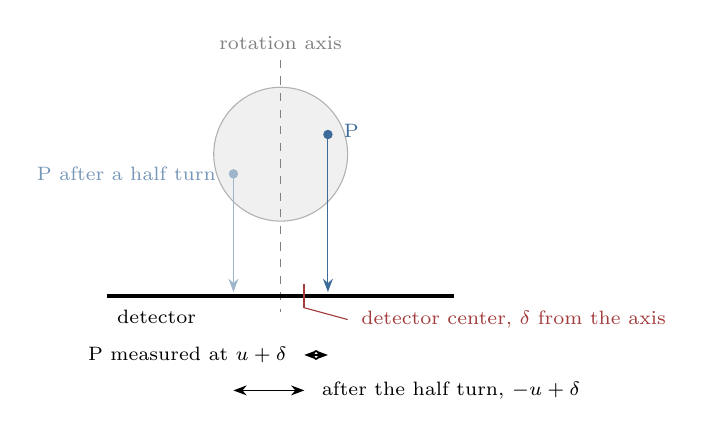
\begin{tikzpicture}[scale=1.0, >=Stealth]
        \draw[fill=gray!12, draw=gray!60] (0,1.1) circle (0.85);
        \draw[dashed, gray] (0,2.3) -- (0,-0.9);
        \node[gray, font=\scriptsize, anchor=south] at (0,2.3) {rotation axis};
        \fill[planAccent] (0.6,1.35) circle (0.06);
        \node[planAccent, font=\scriptsize, anchor=west] at (0.68,1.4) {P};
        \fill[planAccent!50] (-0.6,0.85) circle (0.06);
        \node[planAccent!70, font=\scriptsize, anchor=east] at (-0.7,0.85) {P after a half turn};
        \draw[very thick] (-2.2,-0.7) -- (2.2,-0.7);
        \node[font=\scriptsize, anchor=north west] at (-2.2,-0.75) {detector};
        \draw[->, planAccent] (0.6,1.35) -- (0.6,-0.65);
        \draw[->, planAccent!50] (-0.6,0.85) -- (-0.6,-0.65);
        \draw[thick, axialBrick] (0.3,-0.55) -- (0.3,-0.85);
        \node[axialBrick, font=\scriptsize, anchor=west] at (0.9,-1.0) {detector center, $\delta$ from the axis};
        \draw[axialBrick, thin] (0.3,-0.85) -- (0.85,-1.0);
        \draw[<->, thin] (0.3,-1.45) -- (0.6,-1.45);
        \node[font=\scriptsize, anchor=east] at (0.2,-1.45) {P measured at $u+\delta$};
        \draw[<->, thin] (-0.6,-1.9) -- (0.3,-1.9);
        \node[font=\scriptsize, anchor=west] at (0.4,-1.9) {after the half turn, $-u+\delta$};
      \end{tikzpicture}\\[4pt]
      \figcaption{A point is measured at channel $u+\delta$, and after a half
      turn at $-u+\delta$.  Mirror the second measurement and the two differ
      by $2\delta$, whatever $u$ is.}
    \end{column}
  \end{columns}
  \source{\texttt{mbirtorch/preprocess/geometry\_calibration.py};
  \texttt{docs/source/usr\_preprocess.rst}}
\end{frame}

% ---------------------------------------------------------------- calibration, how well
\begin{continuation}
\begin{frame}{Geometry calibration: how well it works \hfill \released}
  \vspace{0pt}
  \continued{Geometry calibration}{how well the estimators work.}
  \begin{columns}[T]
    \begin{column}{0.52\textwidth}
      {\small \head{Against LEAP on synthetic scans}, 512 and 1024 channels:}\par\vspace{3pt}
      {\footnotesize
      \begin{tabular}{@{}>{\raggedright\arraybackslash}p{0.38\linewidth}@{\hspace{4pt}}>{\raggedright\arraybackslash}p{0.28\linewidth}@{\hspace{4pt}}>{\raggedright\arraybackslash}p{0.28\linewidth}@{}}
        & \speclabel{mbirtorch} & \speclabel{leap} \rowrule
        offset error, inside the search window & within 0.005 channels & up to 0.024 channels \rowrule
        offset outside the default window & failed at 7.5 channels; fixed since, not re-run & found it \rowrule
        rotation error, edge moved over 1.3 pixels & within 0.5 percent & within 1 percent \rowrule
        time for the offset & 0.3 to 4.0 s & 0.1 to 0.9 s \\
      \end{tabular}}
    \end{column}
    \begin{column}{0.46\textwidth}
      {\small \head{On real scans}, four scans of two objects from two
      scanners:}\par\vspace{3pt}
      {\footnotesize
      \begin{itemize}
        \item The offset agreed with the vendors' values to within a tenth of
          a channel.
        \item The estimated rotation is not yet reliable on real scans.  On
          one object it returned 0.047 degrees, where reconstructions are
          sharpest near 0.15 degrees and the vendor recorded 0.167.  The docs
          say to prefer a vendor value; an estimator that scores
          reconstructions is planned.
        \item LEAP's \texttt{estimate\_tilt} found no usable minimum.
      \end{itemize}}
    \end{column}
  \end{columns}
  \source{\texttt{plans/experiments/features/geometric\_calibration/closed/calibration\_512\_gautschi.md} and \texttt{real\_scan\_leap\_tilt.md}}
\end{frame}
\end{continuation}

% ---------------------------------------------------------------- viewer
\begin{frame}{Geometry viewer: see the scan before reconstructing it \hfill \released}
  \begin{columns}[T]
    \begin{column}{0.46\textwidth}
      {\small
      \head{The problem.}  A wrong sign on a detector offset, or a detector
      too small for the object, showed only after a full
      reconstruction.\par\vspace{5pt}
      \head{What changed.}  Five panels draw what the model describes: a 3D
      view, the top and side views, the detector face, and a text panel of
      derived numbers such as the magnification and the fan and cone angles.
      The viewer can overlay a sinogram view and a reconstruction, and draw a
      second geometry over the first with a list of every parameter that
      differs.\par\vspace{5pt}
      \head{How to use it.}\par\vspace{2pt}
      {\scriptsize\ttfamily
      mbirtorch.geometry\_viewer(ct\_model,\\
      \hphantom{mbirt}sinogram=sino, recon=recon,\\
      \hphantom{mbirt}compare=dict(det\_channel\_offset=2.0))\par}}
    \end{column}
    \begin{column}{0.52\textwidth}
      \centering
      \includegraphics[width=\linewidth]{geometry_viewer_cone.png}\\[2pt]
      \figcaption{A cone-beam scan, with a second geometry whose channel
      offset differs drawn over the first in dashed lines.  The sinogram is
      shown on the detector face and the phantom in the volume box.  A slider
      steps through the views.}
    \end{column}
  \end{columns}
  \source{\texttt{mbirtorch/viewers/}; \texttt{docs/source/usr\_geometry\_viewer.rst};
  \texttt{demo/demo\_11\_geometry\_viewer.py}}
\end{frame}

% ---------------------------------------------------------------- geometry rules, 1
\begin{frame}{One geometry map: the problem and what changed \hfill \released}
  \begin{columns}[T]
    \begin{column}{0.54\textwidth}
      {\small
      \head{The problem.}  Each of the four projectors had its own copy of
      the arithmetic that maps a voxel to the detector pixel it lands on.  The
      geometry viewer needs the same map, and a separate copy could disagree
      with the projectors, so the viewer would draw a scan the projectors do
      not compute.\par\vspace{6pt}
      \head{What changed.}  The arithmetic is written once, in
      \texttt{mbirtorch/geometry\_rules.py}.  The projectors' torch code
      calls those functions, and a new method,
      \texttt{TomographyModel.project\_points}, computes the same map for any
      list of points.  The viewer draws through \texttt{project\_points}, so
      it draws what the projectors compute.  The hand-written GPU kernels are
      separate code, checked against the torch code the first time they
      run.\par}
    \end{column}
    \begin{column}{0.44\textwidth}
      \centering
      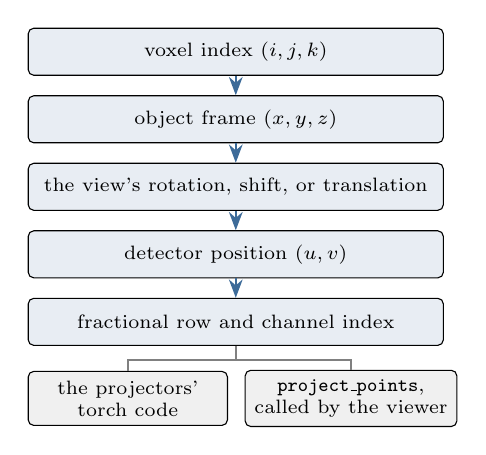
\begin{tikzpicture}[>=Stealth, node distance=7pt,
          box/.style={draw, rounded corners=2pt, fill=planAccent!12, minimum width=150pt, minimum height=17pt, font=\scriptsize, align=center},
          who/.style={draw, rounded corners=2pt, fill=gray!12, minimum width=72pt, minimum height=15pt, font=\scriptsize, align=center}]
        \node[box] (v) {voxel index $(i, j, k)$};
        \node[box, below=of v] (o) {object frame $(x, y, z)$};
        \node[box, below=of o] (r) {the view's rotation, shift, or translation};
        \node[box, below=of r] (d) {detector position $(u, v)$};
        \node[box, below=of d] (p) {fractional row and channel index};
        \draw[->, planAccent, thick] (v) -- (o);
        \draw[->, planAccent, thick] (o) -- (r);
        \draw[->, planAccent, thick] (r) -- (d);
        \draw[->, planAccent, thick] (d) -- (p);
        \node[who, below=9pt of p.south west, anchor=north west] (w1) {the projectors'\\torch code};
        \node[who, right=6pt of w1] (w2) {\texttt{project\_points},\\called by the viewer};
        \draw[gray, thick] (p.south) -- ++(0,-5pt) -| (w1.north);
        \draw[gray, thick] (p.south) ++(0,-5pt) -| (w2.north);
      \end{tikzpicture}\\[4pt]
      \figcaption{One implementation of the map, used by the projectors and,
      through \texttt{project\_points}, by the viewer.}
    \end{column}
  \end{columns}
  \source{\texttt{mbirtorch/geometry\_rules.py}; commits \texttt{d9882d2} and \texttt{511e029}}
\end{frame}

% ---------------------------------------------------------------- geometry rules, 2
\begin{continuation}
\begin{frame}{One geometry map: how to use it \hfill \released}
  \vspace{0pt}
  \continued{One geometry map}{the call a user makes, and the rules as written.}
  \begin{columns}[T]
    \begin{column}{0.54\textwidth}
      {\small
      \head{The map, for points.}
      \texttt{rows, chans = ct\_model.project\_points(points, view)} gives the
      fractional detector indices of object points for one view, by the same
      arithmetic the projectors run.  Integer index $m$ is the center of
      row $m$, and a point off the detector gets an index outside the
      detector; nothing is clipped.\par\vspace{6pt}
      \head{What it is for.}  The viewer's overlays and its comparison of two
      geometries are drawn from it, and a script can use it to check where a
      feature of the object should appear in the sinogram.\par\vspace{6pt}
      \head{The guarantee.}  One implementation, so the viewer's drawing and
      the projectors' computation cannot drift apart.\par}
    \end{column}
    \begin{column}{0.44\textwidth}
      {\small \head{The rules, as written once:}}\par\vspace{4pt}
      {\scriptsize\ttfamily
      x = delta\_voxel * (j - c\_j)\\
      y = delta\_voxel\_row * (i - c\_i)\\
      z = delta\_voxel\_slice * (k - c\_k)\\
      \hphantom{z =} + recon\_slice\_offset\\[6pt]
      channel = (u + det\_channel\_offset)\\
      \hphantom{channel =} / delta\_det\_channel + c\_channel\\
      row = (v + det\_row\_offset)\\
      \hphantom{row =} / delta\_det\_row + c\_row\par}\vspace{6pt}
      \figcaption{Voxel $(i, j, k)$ sits at $(x, y, z)$ in the object frame,
      whose $z$ axis is the rotation axis.  Each $c$ is a center index,
      $(n - 1)/2$ for an axis of length $n$.  A point lands on the detector
      at $(u, v)$, measured from where the central ray meets the detector,
      and the last two rules convert $(u, v)$ to a channel and a row.}
    \end{column}
  \end{columns}
  \source{\texttt{mbirtorch/geometry\_rules.py}; \texttt{mbirtorch/tomography\_model.py}}
\end{frame}
\end{continuation}

% ---------------------------------------------------------------- memory, 1
\begin{frame}{Lower GPU memory: where the memory goes \hfill \released}
  \begin{columns}[T]
    \begin{column}{0.52\textwidth}
      {\small
      \head{The problem.}  On the ORNL scan nvidia-smi showed 39.7 GiB on
      each of four H100 GPUs for mbirtorch, against 6.2 GiB on three of the
      collaborators' four.  On their 40 GB A100s mbirtorch held
      35.6 GB.\par\vspace{6pt}
      \head{Four levels of memory.}  Reading one GPU shows four increasing
      levels, in the order of the chart: the arrays held for the whole run;
      the peak of the arrays in use, reached in the busiest step; the memory
      reserved by the torch allocator, which keeps freed memory for reuse
      instead of returning it to the driver; and the nvidia-smi figure, which
      counts everything the process holds.\par\vspace{6pt}
      \head{What we found.}  The peak came while the error sinogram was
      formed, a step that held five sinogram-sized arrays at once.\par}
    \end{column}
    \begin{column}{0.46\textwidth}
      \centering
      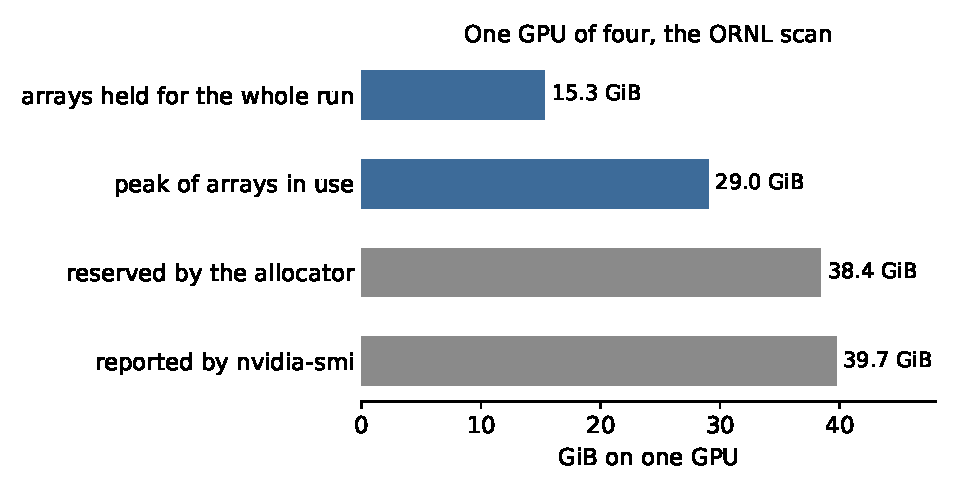
\includegraphics[width=\linewidth]{memory_levels.pdf}\\[2pt]
      \figcaption{The ORNL Inconel scan, 2132 views by 1456 by 1840, on four
      H100 GPUs, 15 iterations, before the changes.}
    \end{column}
  \end{columns}
  \source{\texttt{plans/features/leap\_comparison/ornl\_reproduction.md}, Sections 3.1 and 3.2}
\end{frame}

% ---------------------------------------------------------------- memory, 2
\begin{continuation}
\begin{frame}{Lower GPU memory: what changed and the result \hfill \released}
  \vspace{0pt}
  \continued{Lower GPU memory}{what changed, and the measured result.}
  \begin{columns}[T]
    \begin{column}{0.48\textwidth}
      {\small
      \head{What changed.}  The error sinogram is written into an existing
      array, the sums over the sinogram run in blocks of views, and the
      initial scale needs no sinogram-sized temporary.\par\vspace{5pt}
      \head{The result.}  Arrays in use fell from 29.03 to 24.89 GiB per
      GPU; fifteen iterations took 567.6 s before and 567.9 s after.  The
      memory estimator predicts each step's peak within 1.1 GiB, always on
      the high side.\par\vspace{5pt}
      \head{How to use it.}  Nothing changes.
      \texttt{PYTORCH\_CUDA\_ALLOC\_CONF=expandable\_segments:True} trims the
      freed memory torch keeps; \texttt{mbirtorch.get\_memory\_stats()}
      reports it.\par}
    \end{column}
    \begin{column}{0.50\textwidth}
      \centering
      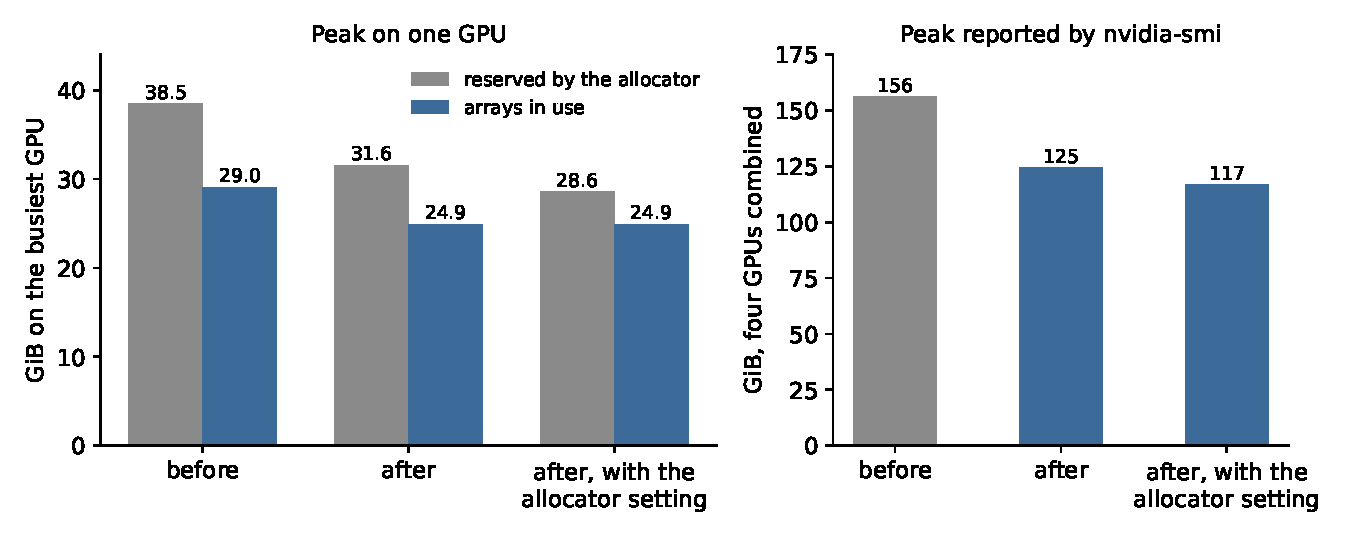
\includegraphics[width=\linewidth]{memory_layers.pdf}\\[2pt]
      \figcaption{The same scan and GPUs, 15 iterations.  The first two bars
      are before and after the three changes; the third bar adds the
      allocator setting.}
    \end{column}
  \end{columns}
  \source{\texttt{plans/experiments/features/device\_memory\_tiers/dm1\_record.md}}
\end{frame}
\end{continuation}

% ---------------------------------------------------------------- gather
\begin{frame}{A reconstruction returns from the GPUs 24 times faster \hfill \released}
  \begin{columns}[T]
    \begin{column}{0.50\textwidth}
      {\small
      \head{The problem.}  A reconstruction split across GPUs must be
      copied back into one host array.  Each GPU holds a range of slices
      along the array's last axis, so its values are not contiguous in the
      host array.  The old copy moved one GPU's slices at a time with one
      host thread: 7.1 to 8.0 s inside a 19.7 s direct reconstruction of the
      ORNL scan.\par\vspace{5pt}
      \head{What changed.}  All GPUs now copy at once, 16 MiB at a time,
      through pinned memory (host memory a GPU can copy to directly), with
      several host threads per GPU.  The result is the same array, byte for
      byte.\par\vspace{5pt}
      \head{How to use it.}  Nothing changes.  \texttt{output\_sharded=True}
      leaves the reconstruction on the GPUs, for when the next step also runs
      there.\par}
    \end{column}
    \begin{column}{0.48\textwidth}
      \centering
      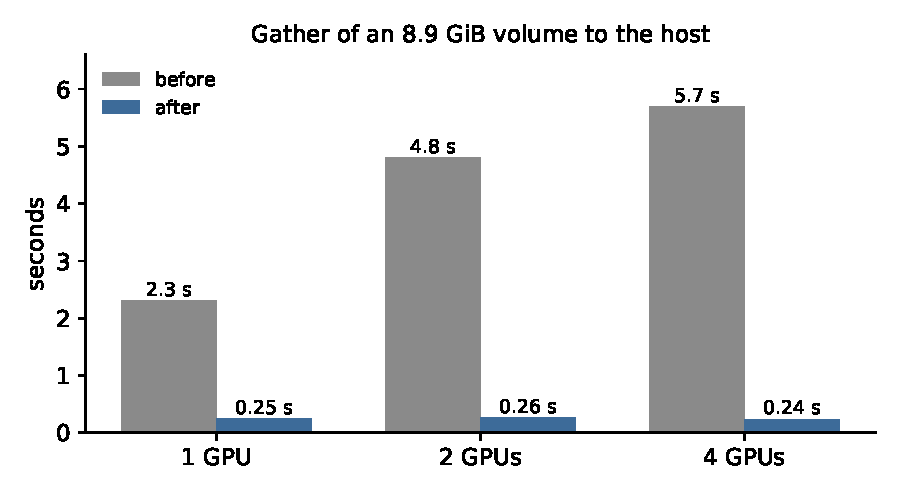
\includegraphics[width=\linewidth]{gather_time.pdf}\\[2pt]
      \figcaption{The ORNL volume, 1360 by 1360 by 1296 float32, 8.9 GiB, on
      gautschi H100 nodes, timed by the gather harness on its own.}
    \end{column}
  \end{columns}
  \source{\texttt{plans/features/leap\_comparison/host\_gather.md};
  \texttt{ornl\_reproduction.md}, Section 3.4}
\end{frame}

% ---------------------------------------------------------------- multiaxis kernels
\begin{frame}{Hand-written kernels for multi-axis parallel beam \hfill \released}
  \begin{columns}[T]
    \begin{column}{0.56\textwidth}
      {\small
      \head{The problem.}  The multi-axis model (laminography, tilted-axis
      scans) ran only through projector code that torch compiles from
      Python.  It needs large temporary arrays, so it was slower and used
      more memory than the other models, more GPUs barely helped, and the
      2048-class size was estimated not to fit on four H100s.\par\vspace{3pt}
      \head{What changed.}  New forward and back kernels in Triton, a language
      for hand-written GPU programs.  They are on by default.\par\vspace{3pt}
      \head{How to use it.}  Nothing;
      \texttt{MBIRTORCH\_DISABLE\_TRITON=1} turns them off.\par\vspace{5pt}
      \footnoteline{The check: at first use on a GPU, once per process, each
      kernel is compared with the torch code on a tiny problem.  The torch
      code takes over only if the two differ by more than 1e-4, which guards
      against a broken compiler on a new machine.}}
    \end{column}
    \begin{column}{0.42\textwidth}
      {\footnotesize \head{The result}, a 1024-class scan of 1024 views by
      1008 rows by 992 channels, three iterations, warm:}\par\vspace{3pt}
      {\footnotesize
      \begin{tabular}{@{}l@{\hspace{5pt}}r@{\hspace{7pt}}r@{\hspace{5pt}}r@{\hspace{5pt}}r@{}}
        & \speclabel{torch code} & \multicolumn{3}{l}{\speclabel{new kernels}} \\
        & \speclabel{1 gpu} & \speclabel{1 gpu} & \speclabel{2 gpus} & \speclabel{4 gpus} \\[2pt]
        time & 309.9 s & 67.6 s & 37.4 s & 22.8 s \\
        memory & 34.8 GB & 24.1 GB & 13.0 GB & 7.5 GB \\
      \end{tabular}}\par\vspace{2pt}
      \figcaption{Memory is the peak of arrays in use on the busiest GPU.
      The kernels are 4.6 times faster on one GPU, and adding GPUs now cuts
      time and memory.}\vspace{4pt}
      \footnoteline{The 2048-class scan, eight times larger at 9.0e9 voxels,
      ran out of memory on two GPUs and completed on four in 298.8 s.  The
      memory estimator, which chooses the GPU count, predicts the kernels'
      memory within 7 percent, so it picks four GPUs for that scan.}
    \end{column}
  \end{columns}
  \source{\texttt{plans/archive/torch\_port/active/multigpu\_findings.md}, Sections 1.45 and 1.46}
\end{frame}

% ---------------------------------------------------------------- smaller changes
\begin{frame}{Smaller changes since the release \hfill \released}
  \vspace{0pt}
  {\footnotesize
  \begin{tabular}{@{}>{\raggedright\arraybackslash}p{0.24\linewidth}@{\hspace{8pt}}>{\raggedright\arraybackslash}p{0.72\linewidth}@{}}
    \speclabel{gpu count} & mbirtorch chooses the number of GPUs from a
      table of problem sizes below which two or four GPUs are slower than
      one.  The table was measured again on the current kernels.
      \texttt{MBIRTORCH\_NUM\_DEVICES} fixes the number instead. \rowrule
    \speclabel{startup} & torch and Triton each save compiled GPU code
      between runs.  Both caches now live in one place, so
      \texttt{mbirtorch.clear\_cache()} clears both.  The input checks read
      each array's minimum and maximum once instead of once per check. \rowrule
    \speclabel{denoiser} & The qGGMRF denoiser keeps \texttt{sigma\_y} equal
      to \texttt{sigma\_noise}, so a user sets the denoising strength with one
      number. \rowrule
    \speclabel{proximal map} & \texttt{prox\_map} now uses
      \texttt{first\_iteration} when a loop calls it again, as a plug-and-play
      loop that alternates the data fit with a denoiser needs. \rowrule
    \speclabel{recon geometry} & A copied model keeps its parent's
      reconstruction shape, pitch, and slice offset; \texttt{build\_model}
      keeps any of those it is given.  The automatic cone and multi-axis
      reconstruction shapes center the volume on the slices the detector rows
      see. \rowrule
    \speclabel{docs and tests} & A geometry viewer page, a calibration section
      in the preprocessing page, and two demos.  The test suite grew from 769
      to 988 functions. \\
  \end{tabular}}
  \source{commits \texttt{9825a43}, \texttt{eee646a}, \texttt{4be9464},
  \texttt{2be05a7}, \texttt{511e029}, \texttt{d7dbd85}, \texttt{41fca86}}
\end{frame}

% ================================================================ transition
\section{Part 1, continued: work not yet in the package}

\begin{frame}{Three features that are complete in code but not released}
  \medskip
  {\small
  The next three slides describe work that a user cannot get from the
  released package today.\par\vspace{8pt}
  \begin{itemize}
    \item \onbranch~\textbf{The MACE loop} is on branch
      \texttt{mace\_4d\_dev}.  Seven commits dated 2026-09-14 add
      \texttt{mbirtorch/mace.py}, \texttt{mbirtorch/mace4d.py}, and 27
      tests.  The documentation, a demo, and an H100 measurement are still
      to be done.\par\vspace{4pt}
    \item \onbranch~\textbf{4D reconstruction} is on the same branch, built
      on the MACE loop.\par\vspace{4pt}
    \item \prototype~\textbf{Multi-slice fusion} runs from research scripts in
      \texttt{experiments/drunet/} and \texttt{mbirtorch\_applications/}.
      It uses the MACE loop, so it enters the package when the loop
      does.\par
  \end{itemize}\vspace{8pt}
  The slides keep the same three parts: the problem, what changed, and how
  to use it.}
  \source{\texttt{plans/features/mace4d/mace4d\_migration\_plan\_v2.md};
  \texttt{plans/nn\_priors/multi\_slice\_fusion.md}}
\end{frame}

% ---------------------------------------------------------------- MACE loop
\begin{frame}{A consensus loop that accepts any agent \hfill \onbranch}
  \begin{columns}[T]
    \begin{column}{0.52\textwidth}
      {\small
      \head{The problem.}  A plug-and-play prior, such as a pretrained
      denoiser, must be combined with the data fit so that the two agree on
      one image.  Every experiment wrote its own loop for that.\par\vspace{6pt}
      \head{What changed.}  One class, \texttt{MACE}, runs multi-agent
      consensus equilibrium.  An agent is any function that takes an image
      array and returns one of the same shape.  Three agents come with it:
      the proximal map of the data term, the qGGMRF denoiser, and a denoiser
      applied along one axis of a stack of images.\par\vspace{6pt}
      \head{How to use it.}\par\vspace{2pt}
      {\scriptsize\ttfamily
      agents = [ForwardProxAgent(model, sino, w),\\
      \hphantom{agents = [}QGGMRFDenoiserAgent(shape, sigma)]\\
      x, info = mace(agents, x0, mu=(0.5, 0.5))\par}}
    \end{column}
    \begin{column}{0.46\textwidth}
      \centering
      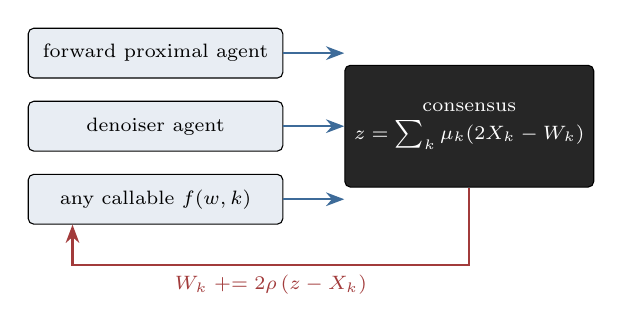
\begin{tikzpicture}[>=Stealth, node distance=8pt and 22pt,
          agent/.style={draw, rounded corners=2pt, fill=planAccent!12, minimum width=92pt, minimum height=18pt, font=\scriptsize},
          cons/.style={draw, rounded corners=2pt, fill=barGray, text=white, minimum width=70pt, minimum height=44pt, font=\scriptsize, align=center}]
        \node[agent] (a1) {forward proximal agent};
        \node[agent, below=of a1] (a2) {denoiser agent};
        \node[agent, below=of a2] (a3) {any callable $f(w, k)$};
        \node[cons, right=of a2] (c) {consensus\\[2pt] $z=\sum_k \mu_k (2X_k - W_k)$};
        \foreach \a in {a1,a2,a3} {
          \draw[->, planAccent, thick] (\a.east) -- (c.west |- \a.east);
        }
        \draw[->, axialBrick, thick] (c.south) -- ++(0,-28pt) -| ($(a3.south)+(-30pt,0)$)
          node[pos=0.25, below, font=\scriptsize, axialBrick] {$W_k \mathrel{+}= 2\rho\,(z - X_k)$};
      \end{tikzpicture}\\[6pt]
      \figcaption{Each agent maps its input $W_k$ to an output $X_k$.  The
      loop forms the consensus point $z$ from the outputs and moves every
      input toward it.  At a fixed point every output equals the weighted
      average of the inputs.}
    \end{column}
  \end{columns}
  \source{\texttt{mbirtorch/mace.py} at \texttt{8304b25}; \texttt{plans/features/mace4d/}}
\end{frame}

% ---------------------------------------------------------------- fusion
\begin{frame}{Multi-slice fusion with a network denoiser \hfill \prototype}
  \begin{columns}[T]
    \begin{column}{0.36\textwidth}
      {\footnotesize
      \head{The problem.}  A pretrained 2D denoiser acts only within its
      own slice plane.  Applied once as postprocessing, it also ignores the
      measured data.\par\vspace{6pt}
      \head{What changed.}  Four MACE agents: the forward proximal map at
      weight 1/2, and one DRUNet denoiser per slice orientation at 1/6 each.
      On a noisy 128-cubed demo scan the NRMSE (error norm over the truth's
      norm) fell from 0.363 to 0.091; one orientation alone gave 0.121, and
      the best postprocessing 0.123.\par\vspace{6pt}
      \head{How to use it.}  Two research scripts, not the package:
      \texttt{nsi/msf\_recon.py}, and \texttt{msf\_ornl.py} for the ORNL
      scan.  The denoiser's noise level sets the strength.\par}
    \end{column}
    \begin{column}{0.62\textwidth}
      \centering
      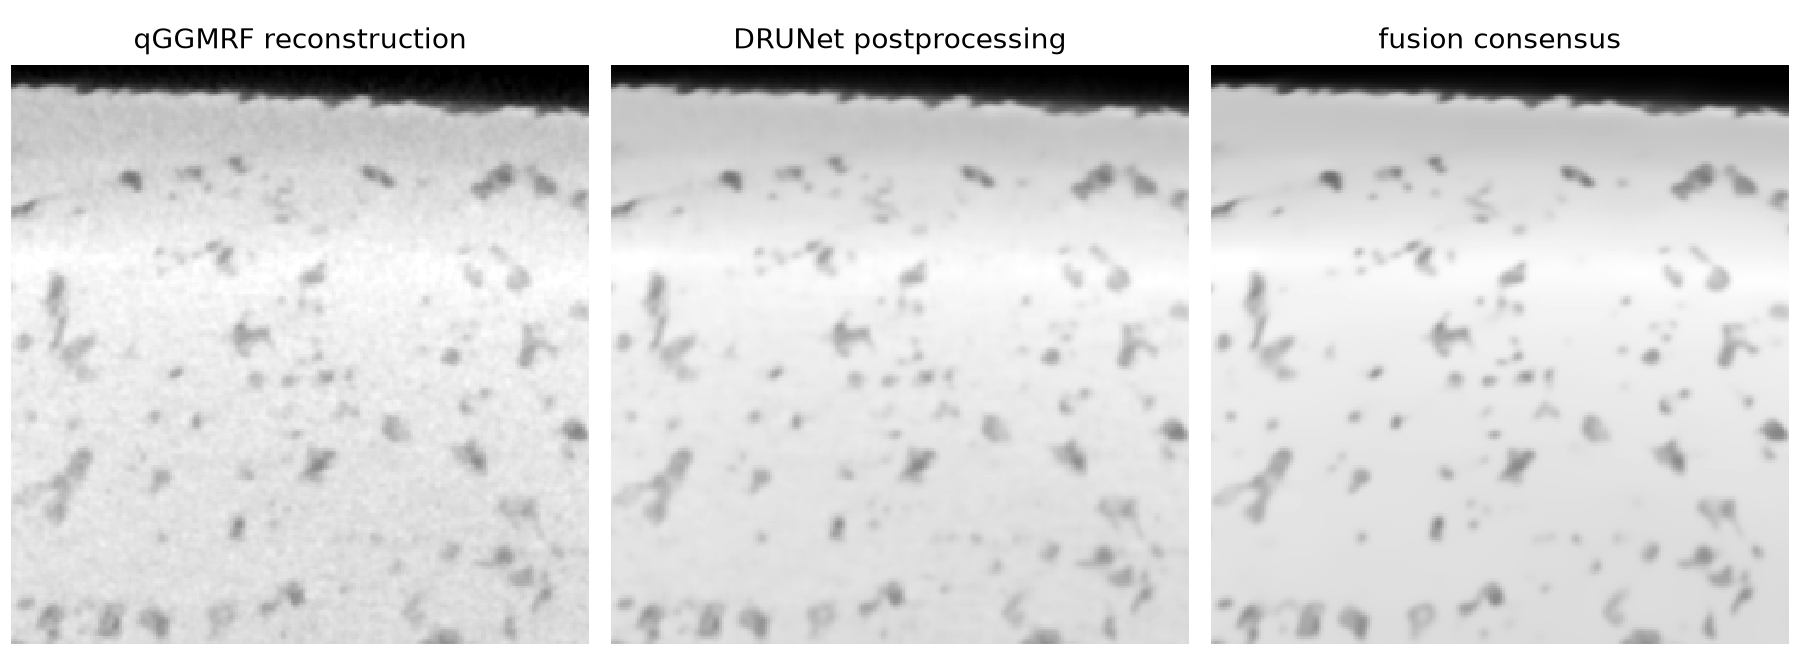
\includegraphics[width=\linewidth]{ornl_fusion_zoom.png}\\[2pt]
      \figcaption{The ORNL Inconel scan, 1360 by 1360 by 1296 voxels: a 240
      by 240 voxel window of one axial slice at the top edge of the part.
      Left: the qGGMRF reconstruction, 15 iterations on four H100s in 619 s,
      41.3 s per iteration averaged over the run, which includes compiling
      the solver and the setup steps.  Middle: DRUNet applied to it slice by
      slice.  Right: the fusion consensus after 25 iterations of 12.3 minutes
      each.  One gray scale for all three.}
    \end{column}
  \end{columns}
  \source{\texttt{plans/nn\_priors/multi\_slice\_fusion\_findings.md};
  \texttt{plans/experiments/features/leap\_comparison/ornl/msf\_ornl.md};
  \texttt{ornl\_reproduction.md}, Section 3.1}
\end{frame}

% ---------------------------------------------------------------- 4D
\begin{frame}{4D reconstruction of a moving object \hfill \onbranch}
  \begin{columns}[T]
    \begin{column}{0.50\textwidth}
      {\small
      \head{The problem.}  When the object moves during one continuous scan,
      one volume cannot represent it, and each time frame reconstructed from
      its few views alone is poor.\par\vspace{4pt}
      \head{What changed.}  \texttt{MACE4DModel} divides the views into
      overlapping angular windows, one per time frame, and reconstructs all
      frames together: each frame's data term is combined with qGGMRF
      denoisers applied in the planes that contain the frame axis, so each
      frame is informed by its neighbors.  A filter along the frame axis then
      removes the periodic variation the overlapping windows
      introduce.\par\vspace{4pt}
      \head{How to use it.}\par\vspace{2pt}
      {\scriptsize\ttfamily
      m4d = MACE4DModel(ct\_model,\\
      \hphantom{m4d = }frames\_per\_rotation=6)\\
      frames = m4d.recon(sino)\par}}
    \end{column}
    \begin{column}{0.48\textwidth}
      \centering
      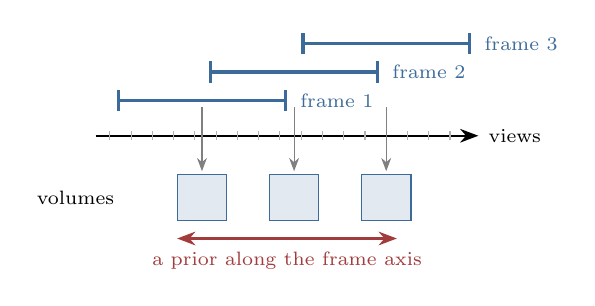
\begin{tikzpicture}[>=Stealth, scale=0.9]
        \draw[->, thick] (0,0) -- (5.4,0) node[right, font=\scriptsize] {views};
        \foreach \x in {0.2,0.5,...,5.1} { \draw[gray!60] (\x,-0.06) -- (\x,0.06); }
        \foreach \i/\y in {0/0.5, 1/0.9, 2/1.3} {
          \pgfmathsetmacro{\xa}{0.3+1.3*\i}
          \pgfmathsetmacro{\xb}{\xa+2.4}
          \draw[planAccent, very thick, |-|] (\xa,\y) -- (\xb,\y);
          \node[planAccent, font=\scriptsize, anchor=west] at (\xb+0.05,\y) {frame \the\numexpr\i+1\relax};
        }
        \foreach \i in {0,1,2} {
          \pgfmathsetmacro{\xc}{0.3+1.3*\i+1.2}
          \draw[->, gray] (\xc,0.4) -- (\xc,-0.5);
          \draw[fill=planAccent!15, draw=planAccent] (\xc-0.35,-1.2) rectangle (\xc+0.35,-0.55);
        }
        \node[font=\scriptsize, anchor=east] at (0.4,-0.87) {volumes};
        \draw[<->, axialBrick, thick] (1.15,-1.45) -- (4.25,-1.45);
        \node[axialBrick, font=\scriptsize, anchor=north] at (2.7,-1.5) {a prior along the frame axis};
      \end{tikzpicture}\\[4pt]
      \figcaption{The views of one continuous scan are divided into
      overlapping angular windows, one per time frame, and one volume is
      reconstructed per frame.}
    \end{column}
  \end{columns}
  \source{\texttt{mbirtorch/mace4d.py} at \texttt{8304b25}; \texttt{plans/features/mace4d/}}
\end{frame}

% ================================================================ PART 2
\section{Part 2: high-value features of LEAP and TIGRE we still lack}

% ---------------------------------------------------------------- evidence
\begin{frame}{How the gaps were found}
  \begin{columns}[T]
    \begin{column}{0.46\textwidth}
      {\small
      \head{Three records.}  A comparison with LEAP, revised this month; the
      same with TIGRE; and a survey of the scripts ORNL collaborators built
      around both packages.\par\vspace{6pt}
      \head{The core algorithm compares well.}  To reach a common image
      quality, VCD, the solver mbirtorch uses, needed 7, 10, and 5 iterations
      at N = 256, 512, and 1024 channels, while LEAP needed 100, 100, and 40.
      mbirtorch's forward and back projectors are exact adjoints of each
      other; LEAP's agree only to the precision of its GPU texture
      interpolation, and TIGRE's are unmatched by design.\par\vspace{6pt}
      \head{So the gaps are in breadth.}  The slides that follow take the
      gaps in order, each starting with what it means for a user.\par}
    \end{column}
    \begin{column}{0.52\textwidth}
      \centering
      \includegraphics[width=\linewidth]{quality_nrmse_vs_time_512.png}\\[2pt]
      \figcaption{The fixed-quality study: both packages reconstruct one
      noisy cone-beam scan from the same data on one H100.  NRMSE is the
      root-mean-square error over the root-mean-square value of the
      reference; the labels are iteration counts.}
    \end{column}
  \end{columns}
  \source{\texttt{plans/features/leap\_comparison/quality\_results.md}; \texttt{leap\_comparison\_v2.md}}
\end{frame}

% ---------------------------------------------------------------- offset scan, 1
\begin{frame}{Offset-scan support \hfill \leaprank{1}~\tigrerank{4}}
  \begin{columns}[T]
    \begin{column}{0.52\textwidth}
      {\footnotesize
      \head{The gap, for a user.}  An offset scan puts the rotation axis
      near one detector edge: each view sees half the object and the views a
      half turn later see the rest, which nearly doubles the width a scanner
      can cover.  mbirtorch cannot reconstruct such a scan correctly
      today.\par\vspace{5pt}
      \head{What LEAP and TIGRE have.}  LEAP weights each channel of an
      offset scan before the ramp filter, so the channels near the axis,
      measured twice, are not counted twice.  TIGRE's FDK does the same by
      default.\par\vspace{5pt}
      \head{What mbirtorch has today.}  The detector offset is a model
      parameter, so the geometry can be described, but nothing weights the
      doubly measured channels.\par\vspace{5pt}
      \head{What's needed.}  A per-channel weight before the ramp filter,
      which the existing filter code can carry, and a check of the iterative
      path on such a scan.\par}
    \end{column}
    \begin{column}{0.46\textwidth}
      \centering
      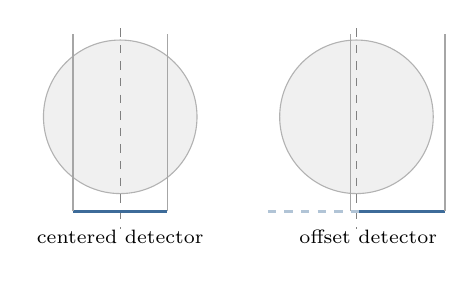
\begin{tikzpicture}[scale=0.75]
        \draw[fill=gray!12, draw=gray!60] (0,1.0) circle (1.3);
        \draw[dashed, gray] (0,2.5) -- (0,-0.9);
        \draw[very thick, planAccent] (-0.8,-0.6) -- (0.8,-0.6);
        \draw[gray!70] (-0.8,-0.6) -- (-0.8,2.4);
        \draw[gray!70] (0.8,-0.6) -- (0.8,2.4);
        \node[font=\scriptsize, anchor=north] at (0,-0.75) {centered detector};
        \begin{scope}[xshift=4.0cm]
          \draw[fill=gray!12, draw=gray!60] (0,1.0) circle (1.3);
          \draw[dashed, gray] (0,2.5) -- (0,-0.9);
          \draw[very thick, planAccent] (-0.1,-0.6) -- (1.5,-0.6);
          \draw[gray!70] (-0.1,-0.6) -- (-0.1,2.4);
          \draw[gray!70] (1.5,-0.6) -- (1.5,2.4);
          \draw[very thick, planAccent!40, dashed] (-1.5,-0.6) -- (0.1,-0.6);
          \node[font=\scriptsize, anchor=north] at (0.2,-0.75) {offset detector};
        \end{scope}
      \end{tikzpicture}\\[4pt]
      \figcaption{Left: an object wider than the detector, so every view is
      cut off at both edges.  Right: the detector shifted until the rotation
      axis sits near one edge.  Each view sees half the object, and the views
      a half turn later see the rest.}
    \end{column}
  \end{columns}
  \source{\texttt{leap\_comparison\_v2.md}, item 1; \texttt{TIGRE\_comparison.md}, item 4}
\end{frame}

% ---------------------------------------------------------------- truncated object
\begin{frame}{Truncated-object support \hfill \leaprank{1}~\tigrerank{4}}
  \begin{columns}[T]
    \begin{column}{0.52\textwidth}
      {\footnotesize
      \head{The gap, for a user.}  Industrial parts are often wider or
      taller than the detector.  A part wider than the detector cannot be
      reconstructed correctly today, and a warning is the only
      sign.\par\vspace{5pt}
      \head{What LEAP has.}  LEAP extends a truncated projection past the
      detector edge before the ramp filter.  For a long object it
      reconstructs the slabs above and below the region and subtracts them
      from the data.\par\vspace{5pt}
      \head{What mbirtorch has today.}  A warning on lateral truncation, and
      \texttt{scale\_recon\_shape} to enlarge the region.  Earlier work on
      axial truncation (an object taller than the detector) handled that half
      on real scans.  The ORNL scripts contain an unused routine that extends
      each projection as the sketch shows.\par\vspace{5pt}
      \head{What's needed.}  The boundary extension before the ramp filter,
      as sketched: repeat the edge value past the detector edge and roll it
      off to zero under a raised cosine.  For a long object, the slab
      method.\par}
    \end{column}
    \begin{column}{0.46\textwidth}
      \centering
      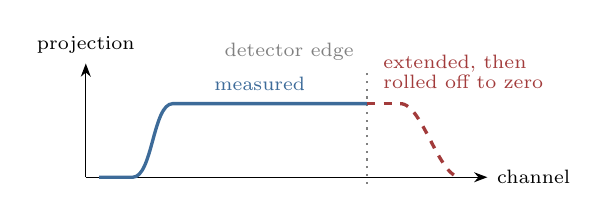
\begin{tikzpicture}[scale=0.85, >=Stealth]
        \draw[->] (0,0) -- (6.0,0) node[right, font=\scriptsize] {channel};
        \draw[->] (0,0) -- (0,1.7) node[above, font=\scriptsize] {projection};
        \draw[dotted, thick, gray] (4.2,-0.1) -- (4.2,1.6);
        \node[gray, font=\scriptsize, anchor=south east] at (4.15,1.6) {detector edge};
        \draw[planAccent, very thick] (0.2,0) -- (0.7,0) .. controls (1.0,0) and (1.0,1.1) .. (1.3,1.1) -- (4.2,1.1);
        \draw[axialBrick, very thick, dashed] (4.2,1.1) -- (4.7,1.1);
        \draw[axialBrick, very thick, dashed, domain=4.7:5.6, samples=30] plot (\x, {1.1*0.5*(1+cos(deg((\x-4.7)/0.9*pi)))});
        \node[planAccent, font=\scriptsize, anchor=south] at (2.6,1.15) {measured};
        \node[axialBrick, font=\scriptsize, anchor=south west] at (4.3,1.42) {extended, then};
        \node[axialBrick, font=\scriptsize, anchor=south west] at (4.3,1.18) {rolled off to zero};
      \end{tikzpicture}\\[4pt]
      \figcaption{One projection of an object that extends past the detector
      edge.  The measured values stop at the edge.  The extension repeats the
      edge value and multiplies it by a raised-cosine taper that falls from
      one to zero, so the ramp filter sees a smooth end instead of a step.
      The ORNL routine does this at both channel edges and both row edges.}
    \end{column}
  \end{columns}
  \source{\texttt{leap\_comparison\_v2.md}, item 1; \texttt{leapMBIR/utils/Get\_projection\_parameters\_standalone\_fast.py:321}}
\end{frame}

% ---------------------------------------------------------------- low memory
\begin{frame}{A low-memory execution mode \hfill \leaprank{2}~\tigrerank{5}}
  \begin{columns}[T]
    \begin{column}{0.50\textwidth}
      {\footnotesize
      \head{The gap, for a user.}  A scan that does not fit the GPUs cannot
      run, and mbirtorch needs more GPU memory than LEAP: on the ORNL scan on
      four H100s it held 39.7 GiB per GPU where the collaborators' LEAP loop
      held 18.9 GiB on one GPU and 6.2 on the other three.\par\vspace{5pt}
      \head{What LEAP and TIGRE have.}  Both chunk each projection operation
      to fit GPU memory, so a large scan runs on small GPUs, at a cost: their
      ORNL loop uses 175 GiB of host memory and spends a third of each
      four-GPU call moving chunks.\par\vspace{5pt}
      \head{What mbirtorch has today.}  The whole problem stays in GPU
      memory, split across the GPUs, so mbirtorch is faster than the chunked
      loop on four GPUs; \texttt{recon\_split\_sino} splits by rows by
      hand.\par}
    \end{column}
    \begin{column}{0.48\textwidth}
      \centering
      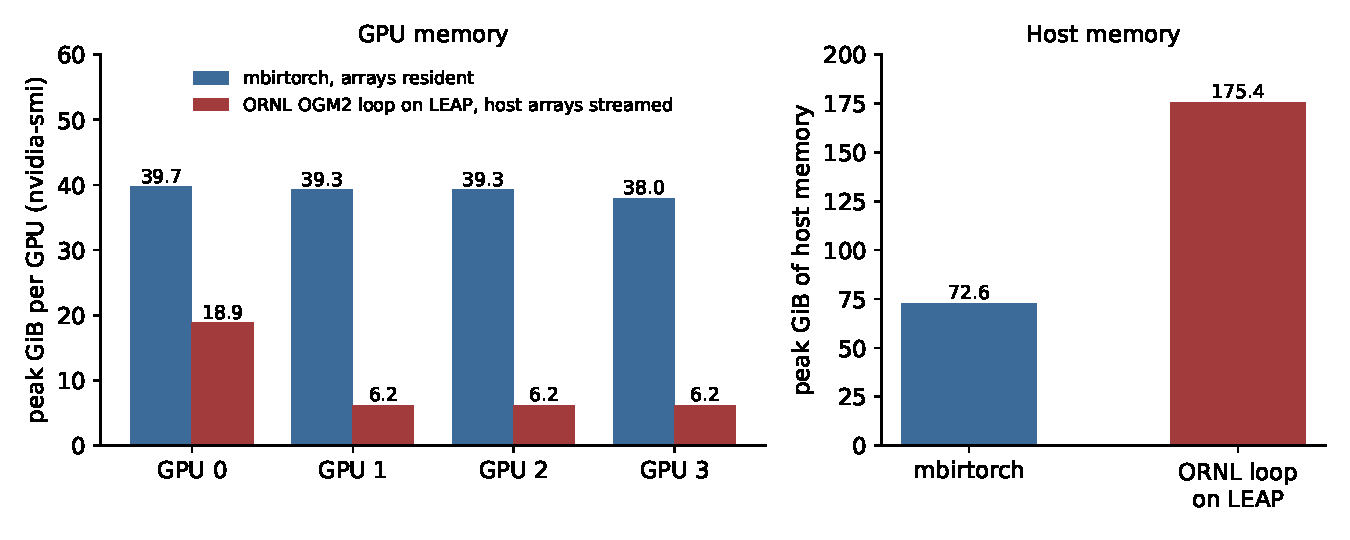
\includegraphics[width=\linewidth]{ornl_gpu_memory.pdf}\\[2pt]
      \figcaption{The ORNL Inconel scan on four H100 GPUs, 15 iterations of
      each loop.  The collaborators' loop keeps every array in host memory
      and streams chunks of at most 128 rows through the GPUs.}
    \end{column}
  \end{columns}
  \vspace{2pt}
  {\footnotesize
  \head{What's needed.}  The device memory tiers plan covers it.  Tier 0,
  the memory saving of slides 9 and 10, is done.  Tier 1, an automatic
  split, reconstructs the sinogram in parts of detector rows and stitches
  them when the whole does not fit at any GPU count.  Tier 2, a host-memory
  mode, keeps the reconstruction-shaped arrays in host memory and streams
  their rows to the GPUs per subset.  Neither is started.\par}
  \source{\texttt{plans/features/leap\_comparison/ornl\_reproduction.md}; \texttt{plans/features/device\_memory\_tiers/}}
\end{frame}

% ---------------------------------------------------------------- physics
\begin{frame}{Scatter correction and spectral physics \hfill \leaprank{3, 5}~\tigrerank{6}}
  \begin{columns}[T]
    \begin{column}{0.48\textwidth}
      {\footnotesize
      \head{The gap, for a user.}  A scan of a large or dense object shows
      cupping and streaks, caused by scatter and beam hardening.  mbirtorch
      has no scatter correction and only an empirical beam-hardening one,
      and quantitative work such as dual-energy decomposition is not
      possible.\par\vspace{5pt}
      \head{What LEAP and TIGRE have.}  See the table.  The ORNL
      collaborators apply LEAP's scatter and beam-hardening corrections to
      every scan they reconstruct.\par\vspace{5pt}
      \head{What mbirtorch has today.}  An empirical beam-hardening curve fit
      and an adaptive correction for objects of plastic and
      metal.\par\vspace{5pt}
      \head{What's needed.}  A constant transmission offset takes a few
      lines of code.  A scatter-kernel estimator needs no spectrum.  The
      physics-based model and the spectral corrections need a spectrum
      library, and the least work is to use an existing one.\par}
    \end{column}
    \begin{column}{0.50\textwidth}
      {\footnotesize
      \begin{tabular}{@{}>{\raggedright\arraybackslash}p{0.34\linewidth}@{\hspace{5pt}}>{\raggedright\arraybackslash}p{0.24\linewidth}@{\hspace{5pt}}>{\raggedright\arraybackslash}p{0.18\linewidth}@{\hspace{5pt}}>{\raggedright\arraybackslash}p{0.16\linewidth}@{}}
        & \speclabel{leap} & \speclabel{tigre} & \speclabel{mbirtorch} \rowrule
        Constant scatter offset & yes & -- & no \rowrule
        Physics-based scatter model & yes, first order & -- & no \rowrule
        Kernel scatter estimator & -- & inside the Varian loader & no \rowrule
        Source spectrum and detector response & yes, through XrayPhysics & -- & no \rowrule
        Beam-hardening correction & spectrum-based & -- & empirical curve fit \rowrule
        Dual-energy decomposition & yes & MATLAB only & no \\
      \end{tabular}}
    \end{column}
  \end{columns}
  \source{\texttt{leap\_comparison\_v2.md}, items 3 and 5; \texttt{TIGRE\_comparison.md}, item 6}
\end{frame}

% ---------------------------------------------------------------- phantoms and noise
\begin{frame}{Analytic phantoms and a noise simulator \hfill \leaprank{4}~\tigrerank{7}}
  \begin{columns}[T]
    \begin{column}{0.50\textwidth}
      {\footnotesize
      \head{The gap, for a user.}  A simulation study in mbirtorch makes its
      data by forward projecting a voxelized phantom with the same model it
      reconstructs with.  That is the inverse crime: it makes the reported
      error lower than the same method gives on real data.  Every study also
      writes its own code to add noise.\par\vspace{5pt}
      \head{What LEAP and TIGRE have.}  LEAP ray-traces a phantom built from
      eight primitive shapes, plus the FORBILD head phantom.  TIGRE adds
      Poisson and Gaussian noise to a set of projections in one call.\par}
    \end{column}
    \begin{column}{0.48\textwidth}
      {\footnotesize
      \head{What mbirtorch has today.}  Voxelized phantom generators, and no
      noise function.\par\vspace{5pt}
      \head{What's needed.}  One ray-intersection routine per primitive
      shape, in the same module as the phantom generators, and one small
      noise function in
      \texttt{mbirtorch/utilities.py}.  The projectors do not
      change.\par\vspace{8pt}
      \noteline{Both items serve method studies.  They rank fourth because
      the prior and fusion results are measured against voxelized phantoms,
      and an analytic phantom would make those comparisons hold up in
      review.}}
    \end{column}
  \end{columns}
  \source{\texttt{leap\_comparison\_v2.md}, item 4; \texttt{TIGRE\_comparison.md}, item 7}
\end{frame}

% ---------------------------------------------------------------- flexible geometry
\begin{frame}{Per-view flexible geometry \hfill \leaprank{6}~\tigrerank{3}}
  \begin{columns}[T]
    \begin{column}{0.50\textwidth}
      {\footnotesize
      \head{The gap, for a user.}  mbirtorch does not allow general per-view
      geometry parameters.  A view can have its own angle, helical shift,
      translation, or elevation, but not its own source position, detector
      position, or detector orientation.  Tomosynthesis, circle-plus-line
      trajectories, detector dithering, and multi-source radiography are
      therefore not possible today.\par\vspace{5pt}
      \head{What LEAP and TIGRE have.}  LEAP's modular beam takes a source
      position, a detector center, and two detector directions per view.
      TIGRE lets three Euler angles, the distances, and the offsets vary per
      view.\par}
    \end{column}
    \begin{column}{0.48\textwidth}
      {\footnotesize
      \head{What mbirtorch has today.}  Per-view angles, helical travel, and
      a per-view elevation in the multi-axis model, which covers
      laminography.\par\vspace{5pt}
      \head{What's needed.}  The largest item on the list.  The
      separable-footprint projector assumes a rotation about a coordinate
      axis, so a general source and detector pose needs either a different
      ray model or a restriction to nearly aligned poses.  It also needs GPU
      kernels, memory estimates, tests, and stored reference values for a
      fifth geometry model, beside cone, parallel, multi-axis, and
      translation.  LEAP's own demo warns that its modular projectors are
      slower and less accurate than its standard ones.\par}
    \end{column}
  \end{columns}
  \source{\texttt{leap\_comparison\_v2.md}, item 6; \texttt{TIGRE\_comparison.md}, item 3}
\end{frame}

% ---------------------------------------------------------------- algorithms and priors
\begin{frame}{Classical algorithms, composable priors, and PICCS \hfill \leaprank{8}~\tigrerank{1, 2}}
  \begin{columns}[T]
    \begin{column}{0.50\textwidth}
      {\footnotesize
      \head{The gap, for a user.}  The author of a paper that uses mbirtorch
      is asked how the method compares with OS-SART, CGLS, or ASD-POCS, and
      must install another package to answer.  Emission or very-low-count
      data need a likelihood that a Gaussian model does not provide.
      Sparse-view data with a prior image, as in 4D reconstruction, has
      PICCS (prior image constrained compressed sensing) as its standard
      baseline.  And mbirtorch has one prior, qGGMRF; a user who wants
      another inside the solver has no way to add it.\par\vspace{5pt}
      \head{What LEAP and TIGRE have.}  LEAP provides twelve iterative
      algorithms, and its \texttt{filterSequence} combines several priors
      inside any of them.  TIGRE provides about two dozen algorithms through
      one interface, and PICCS.\par}
    \end{column}
    \begin{column}{0.48\textwidth}
      {\footnotesize
      \head{What mbirtorch has today.}  VCD with the qGGMRF prior, the
      proximal map, and the MACE loop on a branch, so a total-variation
      prior, a network denoiser, or a prior image can be added to that loop
      as an agent.\par\vspace{5pt}
      \head{What's needed.}  SIRT and OS-SART take a few lines of code on
      top of the existing projectors, and CGLS is a short loop that needs the
      exact adjoint pair mbirtorch has.  A prior built directly into VCD
      needs a new surrogate function, because the update divides by a sum of
      second derivatives and total variation has no second derivative near
      zero.\par}
    \end{column}
  \end{columns}
  \source{\texttt{leap\_comparison\_v2.md}, item 8; \texttt{TIGRE\_comparison.md}, items 1 and 2}
\end{frame}

% ---------------------------------------------------------------- calibration utilities
\begin{frame}{The remaining calibration utilities \hfill \leaprank{7}}
  \begin{columns}[T]
    \begin{column}{0.50\textwidth}
      {\footnotesize
      \head{The gap, for a user.}  mbirtorch has no estimator for a source
      offset from the rotation axis, cannot use a ball phantom to calibrate
      a scanner, and cannot measure resolution.\par\vspace{5pt}
      \head{What LEAP has.}  See the table; TIGRE's center-of-rotation
      estimator exists only in MATLAB.\par\vspace{5pt}
      \head{What mbirtorch has today.}  The two estimators of Part 1, a
      rotation-direction check, a joint search by alternating calls, and
      \texttt{apply\_calibration}, plus a consistency score and a parameter
      sweep that LEAP has no counterpart for.\par\vspace{5pt}
      \head{What's needed.}  The current plan builds an estimator that scores
      reconstructed slices far from the central plane; that measurement
      located the detector rotation on the real scans, and it also works for
      helical and multi-axis scans.  The source offset, the ball phantom, and
      the modulation transfer function (MTF) come after it.\par}
    \end{column}
    \begin{column}{0.48\textwidth}
      {\footnotesize
      \begin{tabular}{@{}>{\raggedright\arraybackslash}p{0.52\linewidth}@{\hspace{5pt}}>{\raggedright\arraybackslash}p{0.18\linewidth}@{\hspace{5pt}}>{\raggedright\arraybackslash}p{0.22\linewidth}@{}}
        & \speclabel{leap} & \speclabel{mbirtorch} \rowrule
        Center of rotation & yes & yes \rowrule
        Detector rotation & yes & yes \rowrule
        Rotation-direction check & no & yes \rowrule
        Applies the estimate & the user does & yes \rowrule
        Source offset \texttt{tau} & yes & no \rowrule
        Inconsistency reconstruction & yes & no \rowrule
        Joint search & yes & alternating calls \rowrule
        Ball-phantom calibration & yes & no \rowrule
        Resolution measurement, MTF & yes & no \\
      \end{tabular}}
    \end{column}
  \end{columns}
  \source{\texttt{leap\_comparison\_v2.md}, the calibration table and item 7;
  \texttt{plans/features/geometric\_calibration/geometric\_calibration\_plan\_v2.md}}
\end{frame}

% ---------------------------------------------------------------- smaller gaps
\begin{frame}{Four smaller gaps \hfill \leaprank{9, 10}~\tigrerank{8, 9}}
  \vspace{0pt}
  {\footnotesize
  \begin{tabular}{@{}>{\raggedright\arraybackslash}p{0.20\linewidth}@{\hspace{8pt}}>{\raggedright\arraybackslash}p{0.48\linewidth}@{\hspace{8pt}}>{\raggedright\arraybackslash}p{0.26\linewidth}@{}}
    \speclabel{gap} & \speclabel{for a user} & \speclabel{what's needed} \rowrule
    A fan-beam model & In mbirtorch a 2D fan-beam dataset is set up as a
      cone-beam model with one detector row.  LEAP has a fan-beam geometry of
      its own. & a small class \rowrule
    Detector deblur & An optics-limited detector, such as the Zeiss Ultra,
      blurs every projection.  LEAP deblurs with a supplied kernel (Wiener
      or Richardson-Lucy). & one preprocessing function \rowrule
    More vendor loaders & TIGRE reads Nikon, Bruker, YXLON, Diondo, DXChange,
      and Varian data.  Neither LEAP nor TIGRE reads the Zeiss Metrotom log
      file that the ORNL scripts parse. & one metadata parser per vendor \rowrule
    A per-iteration quality hook & Every TIGRE algorithm can log RMSE, SSIM,
      and other metrics per iteration; mbirtorch has no hook, so a convergence
      study re-runs the solver at increasing iteration counts. & a callback on \texttt{recon} \\
  \end{tabular}}
  \source{\texttt{leap\_comparison\_v2.md}, items 9 and 10; \texttt{TIGRE\_comparison.md}, items 8 and 9}
\end{frame}

% ---------------------------------------------------------------- summary
\begin{frame}{Summary}
  \vspace{0pt}
  {\small
  \textbf{Since v0.0.2, mbirtorch gained} geometry calibration, a geometry
  viewer, one shared geometry map, lower GPU memory use, a faster return
  from the GPUs, and multi-axis kernels.  On a branch it gained a consensus
  loop and 4D reconstruction; a network-denoiser fusion is a
  prototype.\par\vspace{4pt}
  \textbf{The gaps against LEAP and TIGRE, in order of value:}
  \begin{enumerate}
    \item offset-scan and truncated-object support;
    \item a low-memory execution mode, which the device memory tiers plan
      covers;
    \item scatter correction, starting with a constant offset;
    \item analytic phantoms and a noise simulator, for defensible studies;
    \item polychromatic and dual-energy physics, through a spectrum library;
    \item per-view flexible geometry, the largest item;
    \item classical baselines and prior-image reconstruction, mostly through
      the MACE loop;
    \item the remaining calibration utilities, after the estimator that
      scores reconstructed slices;
    \item a fan-beam model, detector deblur, more loaders, and a quality hook.
  \end{enumerate}}
  \source{\texttt{plans/features/leap\_comparison/leap\_comparison\_v2.md};
  \texttt{plans/features/tigre comparison/TIGRE\_comparison.md}}
\end{frame}

\end{document}
